% This file is part of the i10 thesis template developed and used by the
% Media Computing Group at RWTH Aachen University.
% The current version of this template can be obtained at
% <http://www.media.informatik.rwth-aachen.de/karrer.html>.

\documentclass[11pt, a4paper, titlepage]{book}



% ! ACHTUNG !
% Nach dem ersten LaTeX durchlauf auf der Kommandozeile
% makeindex -s main.ist main.idx
% ausführen, sonst wird der Index nicht so schön formatiert.
% Leider macht TeXShop den makeindex Aufruf nur ohne Parameter.

% !ATTENTION!
% After running LaTeX for the first time using this template call
% makeindex -s main.ist main.idx
% to get the correct formatting for the index.

%Pakete und eigene Befehle - am besten durchlesen!
%Includes all neccessary packets and contains some useful commands - read this file!
% This file is part of the i10 thesis template developed and used by the
% Media Computing Group at RWTH Aachen University.
% The current version of this template can be obtained at
% <http://www.media.informatik.rwth-aachen.de/karrer.html>.



%-----------------------------------------------------------------------------------------------------------------------------------------
% Befehle
% commands
%-----------------------------------------------------------------------------------------------------------------------------------------

%----------------------------------------------------------------------------------
% \myBigFigure	[ LABEL_PREFIX (optional) ]
%				{ FILENAME (without extension) }
%				{ CAPTION TEXT }
%				{ SHORT VERSION OF CAPTION TEXT }
%
%Bild wird in kompletter Breite gesetzt, die Kurzversion der Bildunterschrift erscheint im Abbildungsverzeichnis
%picture using full width of the page, the short caption is what appears in the list of figures index

%----------------------------------------------------------------------------------
% \myFrameBigFigure	[ LABEL_PREFIX (optional) ]
%					{ FILENAME (without extension) }
%					{ CAPTION TEXT }
%					{ SHORT VERSION OF CAPTION TEXT }
%
%Bild wird in kompletter Breite gesetzt und eingerahmt, die Kurzversion der Bildunterschrift erscheint im Abbildungsverzeichnis
%picture with frame using the full width of the page, the short caption is what appears in the list of figures index

%----------------------------------------------------------------------------------
% \myHUGEFigure	[ LABEL_PREFIX (optional) ]
%				{ FILENAME (without extension) }
%				{ CAPTION TEXT }
%				{ SHORT VERSION OF CAPTION TEXT }
%
%Bild wird rotiert und quer in kompletter Breite gesetzt, die Kurzversion der Bildunterschrift erscheint im Abbildungsverzeichnis
%landscape picture using the full width of the rotated page, the short caption is what appears in the list of figures index

%----------------------------------------------------------------------------------
% \myFigure	[ LABEL_PREFIX (optional) ]
%			{ FILENAME (without extension) }
%			{ CAPTION TEXT }
%			{ SHORT VERSION OF CAPTION TEXT }
%
%Bild wird in der Breite der textspalte gesetzt, die Kurzversion der Bildunterschrift erscheint im Abbildungsverzeichnis
%picture using the width of the text column, the short caption is what appears in the list of figures index

%----------------------------------------------------------------------------------
% \myImgRef	[ LABEL_PREFIX (optional) ]
%			{ LABEL OF THE IMAGE }
%
%referenziert das angegebene Bild
%reference to an image

%----------------------------------------------------------------------------------
% \myBigTable	{ YOUR TABULAR DEFINITION }
%			{ CAPTION TEXT }
%			{ TABLE_LABLE }
%
%Tabelle wird in kompletter Breite gesetzt
%table using the full width of the page

%----------------------------------------------------------------------------------
% \myTable	{ YOUR TABULAR DEFINITION }
%			{ CAPTION TEXT }
%			{ TABLE_LABLE }
%
%Tabelle wird in der Breite der Textspalte gesetzt
%table using the width of the text column

%----------------------------------------------------------------------------------
% \myTxtRef	{ LABLE }
%
%Referenz auf Kapitel oder Abschnitte - gibt nummer und namen aus, z.B.: 5.3---"Yaddahyaddah"
%references chapters or sections, outputs number and title, e.g., 5.3---"Yaddahyaddah"

%----------------------------------------------------------------------------------
% \myUnderscore
%
%Setzt einen "sch�nen" Unterstrich f�r URLs
%typesets a 'nice' underscore for URLs

%----------------------------------------------------------------------------------
%\myTilde
%
%Setzt eine "sch�ne" Tilde f�r URLs
%typesets a 'nice' tilde for URLs

%----------------------------------------------------------------------------------
% \myURL	{ TYPESET VERSION OF ANCHOR }
%			{ PRISTINE URL }
%			{ TYPESET VERSION OF URL }
%
%Setzt eine URL
%die typographisch "sch�ne" version erscheint in einer Fu�note,
%im Text erscheint der Ankertext, verlinkt ist die "echte" URL
%typesets a URL
%the typographically correct version appears as a footnote,
%the anchor appears in the text, the link points to the pristine URL

%----------------------------------------------------------------------------------
% \mySimpleURL	{ TYPESET VERSION OF ANCHOR }
%				{ PRISTINE URL }
%
%Setzt eine URL
%die URL erscheint in einer Fu�note,
%im Text erscheint der Ankertext, die URL ist verlinkt
%typesets a URL
%the URL appears as a footnote,
%the anchor appears in the text, the link points to the URL

%----------------------------------------------------------------------------------
% \myProjectURL	{ TYPESET VERSION OF ANCHOR }
%				{ PRISTINE URL INSIDE PROJECT DIRECTORY }
%				{ TYPESET VERSION OF URL INSIDE PROJECT DIRECTORY }
%
%Setzt eine URL innerhalb des Projektverzeichnisses auf "media"
%ACCOUNT muss durch den eigenen Usernamen ersetzt werden
%die typographisch "sch�ne" version erscheint in einer Fu�note,
%im Text erscheint der Ankertext, verlinkt ist die "echte" URL
%typesets a URL inside the project directory on 'media'
%replace ACCOUNT with your username
%the typographically correct version appears as a footnote,
%the anchor appears in the text, the link points to the pristine URL

%----------------------------------------------------------------------------------
% \mnote	{ MARGIN NOTE }
%
%Setzt eine Randnotitz
%puts a comment into the margin in small sans-serif font

%----------------------------------------------------------------------------------
% \todo	{ TODO MARGIN NOTE }
%
%Setzt eine "ToDo"-Randnotitz in rot zur Erinnerung
%puts a 'todo' comment into the margin in red

%----------------------------------------------------------------------------------
% \chapterquote	{ QUOTATION }
%				{ SOURCE }
%
%Setzt ein Zitat zum Einleiten eines Kapitels
%outputs a quote with its source, can be used as an introduction to chapters

%----------------------------------------------------------------------------------
% \myDefBox	{ TERM }
%			{ DEFINITION }
%
%Setzt eine Randnotitz und eine farbige Box (Textspaltenbreite),
%welche einen Begriff und seine Definition enth�lt
%outputs a margin note and a colored box (width of the text column) containing a term and its definition

%----------------------------------------------------------------------------------
% \myBigDefBox	{ TERM }
%				{ DEFINITION }
%
%Setzt eine farbige Box (Seitenbreite), welche einen Begriff und seine Definition enth�lt
%outputs a colored box (width of the page) containing a term and its definition

%----------------------------------------------------------------------------------
% \myDownloadURL	{ TYPESET DOWNLOAD NAME }
%					{ PRISTINE VERSION OF FILENAME }
%					{ TYPESET VERSION OF FILENAME }
%
%Setzt eine farbige Box, welche einen Downloadlink enth�lt
%outputs a colored box containing a download link

%----------------------------------------------------------------------------------
% \emptydoublepage
%
% Leere Doppelseite ohne Kopf- oder Fu�zeile am Ende von Kapiteln
% Clear double page without any header or footer at end of chapters

%----------------------------------------------------------------------------------
% \pagebreak	[ SOME STRANGE LATEX VALUE ]
%
%Eklige pagebreaks f�r den Druck (falls es nicht mehr anders geht)
%pagebreaks for the final print version (last resort weapon against wrong pagebreaks by LaTeX)



%----------------------------------------------------------------------------------
%Packages and parameters
%----------------------------------------------------------------------------------

%Inputencoding f�r den Mac
%inputencoding for the mac
\usepackage[ngerman]{babel}
\usepackage[utf8]{inputenc}
\usepackage[T1]{fontenc}
\usepackage{lmodern}
\usepackage{acronym}


%Mathe- und Symbolpakete
%packages for mathematical symbols
\usepackage{latexsym}
\usepackage{amsmath}
\usepackage{amssymb}

%Grafikpaket
%grahics package
\usepackage{color,graphicx}

%relativer Pfad zu den Bildern
%path to your image folder
\graphicspath{{images/}}

%Abs�tze werden nicht eingezogen, sondern vertikal abgesetzt
%do not indent at new paragraphs but add a vertical offset
\usepackage{noindent}

%Palatino+Helvetica statt Computer Modern als standard fonts:
%change standard fonts to Palatino and Helvetica
\usepackage{palatino}

%Bibliographieeinstellungen
%bibliography settings
\usepackage{natbib}
\bibliographystyle{plainnat}

%Zitierbefehle
%citation commands
\newcommand{\fullcite}{\citep} %for "Author [1980]"
\renewcommand{\citeyear}{\citeyearpar} %for "[1980]"

%paket f�r erweiterte kontrollstrukturen
%package for control structures
\usepackage{ifthen}

%marginpar hack --- alle Randnotitzen sollten dann auf der richtigen Seite stehen
%marginpar hack --- moves margin notes to correct position
\usepackage{mparhack}

%lesbare verweise
%make readable references
\usepackage[pdftex,plainpages=false,pdfpagelabels]{hyperref}


%---------------------<Layout in the style of "A Pattern Approach to Interaction Design>---------------------------

% Change page headers and footers:
\usepackage{fancyhdr}
\pagestyle{fancy}
\fancyhf{}
\fancyhead[RE]{\slshape \nouppercase{\leftmark}}    % Even page header: "page   chapter"
\fancyhead[LO]{\slshape \nouppercase{\rightmark}}   % Odd  page header: "section   page"
\fancyhead[RO,LE]{\bfseries \thepage} 
\renewcommand{\headrulewidth}{1pt}    % Underline headers
\renewcommand{\footrulewidth}{0pt}    

\fancypagestyle{plain}{               % No chapter+section on chapter start pages
\fancyhf{}
\fancyhead[RO,LE]{\bfseries \thepage}
\renewcommand{\headrulewidth}{1pt}
\renewcommand{\footrulewidth}{0pt}
}

% Left headings: "1  INTRODUCTION"
\renewcommand{\chaptermark}[1]{%
\markboth{\thechapter\ \ \ \ #1}{}}

% Right headings: "1.1  Basics"
\renewcommand{\sectionmark}[1]{%
\markright{\thesection\ \ \ \ #1}{}}


% Page layout
\topmargin20mm
\addtolength{\headheight}{2pt} % To avoid overfull vboxes from fancyhdr
\footskip10mm % space text bottom <-> date stamp

\oddsidemargin5mm
\evensidemargin30mm

\textwidth130mm
\marginparsep10mm
\marginparwidth30mm


\newlength{\fullwidth} % Width of text plus margin notes
\setlength{\fullwidth}{\textwidth}
\addtolength{\fullwidth}{\marginparsep}
\addtolength{\fullwidth}{\marginparwidth}


\setlength{\headwidth}{\fullwidth} % Header stretches over margin notes


%---------------------</Layout in the style of "A Pattern Approach to Interaction Design>---------------------------


%wird f�r die fl�chendeckende Ausgabe der Titelseite ben�tigt
%needed for the full-face titlepage
\usepackage{eso-pic}

%index verwenden
%make an index
\usepackage{makeidx}
\makeindex

%Index Formatierungshilfen
%formatting helpers for the index
\newcommand{\uu}[1]{\underline{#1}}
\newcommand{\ii}[1]{\textit{#1}}

%neue Definition der Index Umgebung
%redesign of the index
\renewenvironment{theindex}{%
  \vspace*{50pt}%
  {\Huge\bfseries\indexname}\par%
  \vspace*{40pt}%
  \setlength{\parskip}{0pt}%
  \setlength{\parindent}{0pt}%
  \small%
  \renewcommand{\item}{\par{}}%
  \renewcommand{\subitem}{\par\hspace{2em}- }%
}%
{}

%Maximale Gliederungstiefe, die noch ins Inhaltsverzeichnis aufgenommen wird
%maximum depth for the table of contents
\setcounter{tocdepth}{3}

%Vorschlag f�r ein sch�nes Farbschema
%Set of colors which look nice together
\usepackage{color}
\definecolor{orange_light}{rgb}{1,0.8,0.4}
\definecolor{orange_med}{rgb}{0.753,0.62,0.373}
\definecolor{orange_dark}{rgb}{0.506,0.412,0.251}

\definecolor{green_light}{rgb}{0.8,1,0.4}
\definecolor{green_med}{rgb}{0.635,0.745,0.376}
\definecolor{green_dark}{rgb}{0.435,0.498,0.255}

\definecolor{blue_light}{rgb}{0.4,0.8,1}
\definecolor{blue_med}{rgb}{0.365,0.624,0.749}
\definecolor{blue_dark}{rgb}{0.251,0.42,0.502}

\definecolor{pink_light}{rgb}{1,0.435,0.812}
\definecolor{pink_med}{rgb}{0.745,0.38,0.62}
\definecolor{pink_dark}{rgb}{0.498,0.255,0.416}

\definecolor{yellow_light}{rgb}{1,1,0.4}
\definecolor{yellow_med}{rgb}{0.757,0.745,0.373}
\definecolor{yellow_dark}{rgb}{0.506,0.49,0.251}

%blau (f�r URLs)
%blue (for URLs)
\definecolor{blue}{rgb}{0,0,1}

%notwendig f�r die korrekte Erkennung, auf welcher Seite sich eine Abbildung befindet.
%we need this to determine if a figure is on an odd or even page
\usepackage{chngpage}

%Hiermit k�nnen die Abbildungslegenden frei gestaltet werden
%we need this to redesign the captions
\usepackage[font=normalsize,labelfont=bf]{caption}

%Abbildungen kommen auf eine eigene Seite, wenn sie mehr als 85% des Platzes
%auf einer Seite einnehmen
%if a figure takes more than 85% of a page it will be typeset on a separate page
\renewcommand{\floatpagefraction}{0.85}

%Ben�tigt um gro�e Abbildungen gedreht auf eine Seite zu setzen
%we need this to rotate big figures
\usepackage[figuresright]{rotating}

%Verschiedene L�ngenma�e f�r Textboxen
%dimensions for textboxes
\newlength{\myDefBoxWidth}
\setlength{\myDefBoxWidth}{\textwidth}
\addtolength{\myDefBoxWidth}{-4mm}
\newlength{\myBigDefBoxWidth}
\setlength{\myBigDefBoxWidth}{\fullwidth}
\addtolength{\myBigDefBoxWidth}{-4mm}

%Formathilfen f�r MatLab Code (wer's braucht...)
%pre-defined matlab code formats
\usepackage{alltt}
\definecolor{string}{rgb}{0.7,0.0,0.0}
\definecolor{comment}{rgb}{0.13,0.54,0.13}
\definecolor{keyword}{rgb}{0.0,0.0,1.0}



%-----------------------------------------------------------------------------------------------------------------------------------------
% neue Befehle
% new commands
%-----------------------------------------------------------------------------------------------------------------------------------------

%----------------------------------------------------------------------------------
% \myBigFigure	[ LABEL_PREFIX (optional) ]
%				{ FILENAME (without extension) }
%				{ CAPTION TEXT }
%				{ SHORT VERSION OF CAPTION TEXT }
%
%Bild wird in kompletter Breite gesetzt
%picture using full width of the page
\newcommand{\myBigFigure}[4][image]
{
\begin{figure}[t!bp]
	\checkoddpage
	\ifcpoddpage
		%nothing
	\else
		\hspace{-\marginparsep}\hspace{-\marginparwidth}
	\fi
	%use minipage to center the label beneath the figure
	\begin{minipage}{\fullwidth}
		\includegraphics[width= \fullwidth]{#2}
		\caption[#4]{#3}
		\label{#1_#2}
	\end{minipage}
\end{figure}
}


%----------------------------------------------------------------------------------
% \myFrameBigFigure	[ LABEL_PREFIX (optional) ]
%					{ FILENAME (without extension) }
%					{ CAPTION TEXT }
%					{ SHORT VERSION OF CAPTION TEXT }
%
%Bild wird in kompletter Breite gesetzt und eingerahmt
%picture with frame using the full width of the page
\newcommand{\myFrameBigFigure}[4][image]
{
\begin{figure}[t!bp]
	\checkoddpage
	\ifcpoddpage
		%nothing
	\else
		\hspace{-\marginparsep}\hspace{-\marginparwidth}
	\fi
	%use minipage to center the label beneath the figure
	\begin{minipage}{\fullwidth}
	\frame{%
		\includegraphics[width= \fullwidth]{#2}%
		}
		\caption[#4]{#3}
		\label{#1_#2}
	\end{minipage}
\end{figure}
}

%----------------------------------------------------------------------------------
% \myHUGEFigure	[ LABEL_PREFIX (optional) ]
%				{ FILENAME (without extension) }
%				{ CAPTION TEXT }
%				{ SHORT VERSION OF CAPTION TEXT }
%
%Bild wird rotiert und quer in kompletter Breite gesetzt
%landscape picture using the full width of the rotated page
\newcommand{\myHugeFigure}[4][image]
{
\begin{sidewaysfigure}[t!bp]
	
		\includegraphics[width= \textheight]{#2}
		\caption[#4]{#3}
		\label{#1_#2}
	
\end{sidewaysfigure}
}

%----------------------------------------------------------------------------------
% \myFigure	[ LABEL_PREFIX (optional) ]
%			{ FILENAME (without extension) }
%			{ CAPTION TEXT }
%			{ SHORT VERSION OF CAPTION TEXT }
%
%Bild wird in der Breite der textspalte gesetzt
%picture using the width of the text column
\newcommand{\myFigure}[4][image]%
{%
\begin{figure}[ht!bp]%
	\begin{center}%
		\includegraphics[width= \textwidth]{#2}%
		\caption[#4]{#3}
		\label{#1_#2}%
	\end{center}%
\end{figure}%
}%

%----------------------------------------------------------------------------------
% \myImgRef	[ LABEL_PREFIX (optional) ]
%			{ LABEL OF THE IMAGE }
%
%referenziert das angegebene Bild
%reference to an image
\newcommand{\myImgRef}[2][image]%
{%
	\ref{#1_#2}%
}%

%----------------------------------------------------------------------------------
% \myBigTable	{ YOUR TABULAR DEFINITION }
%			{ CAPTION TEXT }
%			{ TABLE_LABLE }
%
%Tabelle wird in kompletter Breite gesetzt
%table using the full width of the page
\newcommand{\myBigTable}[3]%
{%
\begin{table}[htdp]%
	\checkoddpage%
	\ifcpoddpage%
		%nothing
	\else%
		\hspace{-\marginparsep}\hspace{-\marginparwidth}%
	\fi%
	\begin{minipage}{\fullwidth}%
		\begin{center}%
			#1%
			\caption{#2}%
			\label{#3}%
		\end{center}%	
	\end{minipage}%
\end{table}%
}%

%----------------------------------------------------------------------------------
% \myTable	{ YOUR TABULAR DEFINITION }
%			{ CAPTION TEXT }
%			{ TABLE_LABLE }
%
%Tabelle wird in der Breite der Textspalte gesetzt
%table using the width of the text column
\newcommand{\myTable}[3]%
{%
\begin{table}[htdp]%
	\begin{center}%
		#1%
		\caption{#2}%
		\label{#3}%
	\end{center}%	
\end{table}%
}%

%----------------------------------------------------------------------------------
% \myTxtRef	{ LABLE }
%
%Referenz auf Kapitel oder Abschnitte - gibt nummer und namen aus, z.B.: 5.3---"Yaddahyaddah"
%references chapters or sections, outputs number and title, e.g., 5.3---"Yaddahyaddah"
\newcommand{\myTxtRef}[1]
{%
	\ref{#1}---``\nameref{#1}''%
}

%----------------------------------------------------------------------------------
% \myUnderscore
%
%Setzt einen "sch�nen" Unterstrich f�r URLs
%typesets a 'nice' underscore for URLs
\newcommand{\myUnderscore}{$\underline{\hspace{0.5em}}$}

%----------------------------------------------------------------------------------
%\myTilde
%
%Setzt eine "sch�ne" Tilde f�r URLs
%typesets a 'nice' tilde for URLs
\newcommand{\myTilde}{$\sim$}

%----------------------------------------------------------------------------------
% \myURL	{ TYPESET VERSION OF ANCHOR }
%			{ PRISTINE URL }
%			{ TYPESET VERSION OF URL }
%
%Setzt eine URL
%die typographisch "sch�ne" version erscheint in einer Fu�note,
%im Text erscheint der Ankertext, verlinkt ist die "echte" URL
%typesets a URL
%the typographically correct version appears as a footnote,
%the anchor appears in the text, the link points to the pristine URL
\newcommand{\myURL}[3]%
{%
	\textcolor{blue}{%
		\href{#2}{#1}%
	}%
	\footnote{#3}
}

%----------------------------------------------------------------------------------
% \mySimpleURL	{ TYPESET VERSION OF ANCHOR }
%				{ PRISTINE URL }
%
%Setzt eine URL
%die URL erscheint in einer Fu�note,
%im Text erscheint der Ankertext, die URL ist verlinkt
%typesets a URL
%the URL appears as a footnote,
%the anchor appears in the text, the link points to the URL
\newcommand{\mySimpleURL}[2]%
{%
	\textcolor{blue}{%
		\href{#2}{#1}%
	}%
	\footnote{#2}
}

%----------------------------------------------------------------------------------
% \myProjectURL	{ TYPESET VERSION OF ANCHOR }
%				{ PRISTINE URL INSIDE PROJECT DIRECTORY }
%				{ TYPESET VERSION OF URL INSIDE PROJECT DIRECTORY }
%
%Setzt eine URL innerhalb des Projektverzeichnisses auf "media"
%ACCOUNT muss durch den eigenen Usernamen ersetzt werden
%die typographisch "sch�ne" version erscheint in einer Fu�note,
%im Text erscheint der Ankertext, verlinkt ist die "echte" URL
%typesets a URL inside the project directory on 'media'
%replace ACCOUNT with your username
%the typographically correct version appears as a footnote,
%the anchor appears in the text, the link points to the pristine URL
\newcommand{\myProjectURL}[3]%
{%
	\textcolor{blue}{%
		\href{http://media.informatik.rwth-aachen.de/~ACCOUNT/thesis/#2}{#1}%
	}%
	\footnote{http://media.informatik.rwth-aachen.de/\myTilde ACCOUNT/thesis/#3}%
}

%----------------------------------------------------------------------------------
% \mnote	{ MARGIN NOTE }
%
%Setzt eine Randnotitz
%puts a comment into the margin in small sans-serif font
\newcommand{\mnote}[1]{\marginpar{\raggedright\textsf{{\footnotesize{#1}}}}}

%----------------------------------------------------------------------------------
% \todo	{ TODO MARGIN NOTE }
%
%Setzt eine "ToDo"-Randnotitz in rot zur Erinnerung
%puts a 'todo' comment into the margin in red
\definecolor{red}{rgb}{1,0,0}
\newcommand{\todo}[1]{\mnote{\textcolor{red}{ToDo: #1}}}

%----------------------------------------------------------------------------------
% \chapterquote	{ QUOTATION }
%				{ SOURCE }
%
%Setzt ein Zitat zum Einleiten eines Kapitels
%outputs a quote with its source, can be used as an introduction to chapters
\newcommand{\chapterquote}[2]{
\begin{quotation}
    \begin{flushright}
	\noindent\emph{``{#1}''\\[1.5ex]---{#2}}
    \end{flushright}
\end{quotation}
}

%----------------------------------------------------------------------------------
% \myDefBox	{ TERM }
%			{ DEFINITION }
%
%Setzt eine Randnotitz und eine farbige Box (Textspaltenbreite),
%welche einen Begriff und seine Definition enth�lt
%outputs a margin note and a colored box (width of the text column) containing a term and its definition
\newcommand{\myDefBox}[2]
{%
	\setlength{\fboxrule}{1mm}%
	\fcolorbox{orange_med}{orange_light}%
	{%
		\parbox{\myDefBoxWidth}{{\bfseries\scshape#1:}\\#2}%
	}%
	\mnote{Definition:\\\emph{#1}}
}

%----------------------------------------------------------------------------------
% \myBigDefBox	{ TERM }
%				{ DEFINITION }
%
%Setzt eine farbige Box (Seitenbreite), welche einen Begriff und seine Definition enth�lt
%outputs a colored box (width of the page) containing a term and its definition
\newcommand{\myBigDefBox}[2]
{%
	\begin{figure}[h!]
	\setlength{\fboxrule}{1mm}%
	\checkoddpage%
	\ifcpoddpage%
		%nothing
	\else%
		\hspace{-\marginparsep}\hspace{-\marginparwidth}%
	\fi%
	\fcolorbox{orange_med}{orange_light}%
	{%
		\parbox{\myBigDefBoxWidth}{{\bfseries\scshape#1:}\\#2}%
	}%
	\end{figure}
}

%----------------------------------------------------------------------------------
% \myDownloadURL	{ TYPESET DOWNLOAD NAME }
%					{ PRISTINE VERSION OF FILENAME }
%					{ TYPESET VERSION OF FILENAME }
%
%Setzt eine farbige Box, welche einen Downloadlink enth�lt
%outputs a colored box containing a download link
\newcommand{\myDownloadURL}[3]{%
\checkoddpage%
	\ifcpoddpage%
		%nothing
	\else%
		\hspace{-\marginparsep}\hspace{-\marginparwidth}%
	\fi%
\setlength{\fboxrule}{1mm}%
\fcolorbox{green_med}{green_light}{%
\begin{minipage}{\myBigDefBoxWidth}%
\begin{center}%
\myProjectURL{#1}{folder/#2}{folder/#3}%
\end{center}%
\end{minipage}%
}%
}

%----------------------------------------------------------------------------------
% \emptydoublepage
%
% Leere Doppelseite ohne Kopf- oder Fu�zeile am Ende von Kapiteln
% Clear double page without any header or footer at end of chapters
\newcommand{\emptydoublepage}{\clearpage\thispagestyle{empty}\cleardoublepage}

%----------------------------------------------------------------------------------
% \pagebreak	[ SOME STRANGE LATEX VALUE ]
%
%Eklige pagebreaks f�r den Druck (falls es nicht mehr anders geht)
%pagebreaks for the final print version (last resort weapon against wrong pagebreaks by LaTeX)
\newcommand{\PB}[1][3]
{%
	\pagebreak[#1]%
}



%--------------------------------------------------------------
%Dokumentspezifisches
%Stuff regarding your specific document
%--------------------------------------------------------------

%Trennungshilfen
%Hyphenation patterns
\hyphenation{
dieseswortwirdnichtgetrennt
diesesauchnicht
thiswordwillstayinoneline
thistoo
}


%--------------------------------------------------------------
\begin{document}

% größere Wortabstände zulassen, um Trennungen zu vermeiden
% allow more flexible whitespaces to avoid hyphenation and overfull hboxes
\sloppy

% "see" Einträge für den Index
% 'see'-entries for the index
% This file is part of the i10 thesis template developed and used by the
% Media Computing Group at RWTH Aachen University.
% The current version of this template can be obtained at
% <http://www.media.informatik.rwth-aachen.de/karrer.html>.

\index{abbrv|see{abbreviation}}




%--------------------------------------------------------------
\frontmatter

%Die Titelseite aus dem "images"-Verzeichnis wird verwendet
%use the titlepage from the 'images' directory 
\begin{titlepage}
\AddToShipoutPicture*{
\put(0,0){
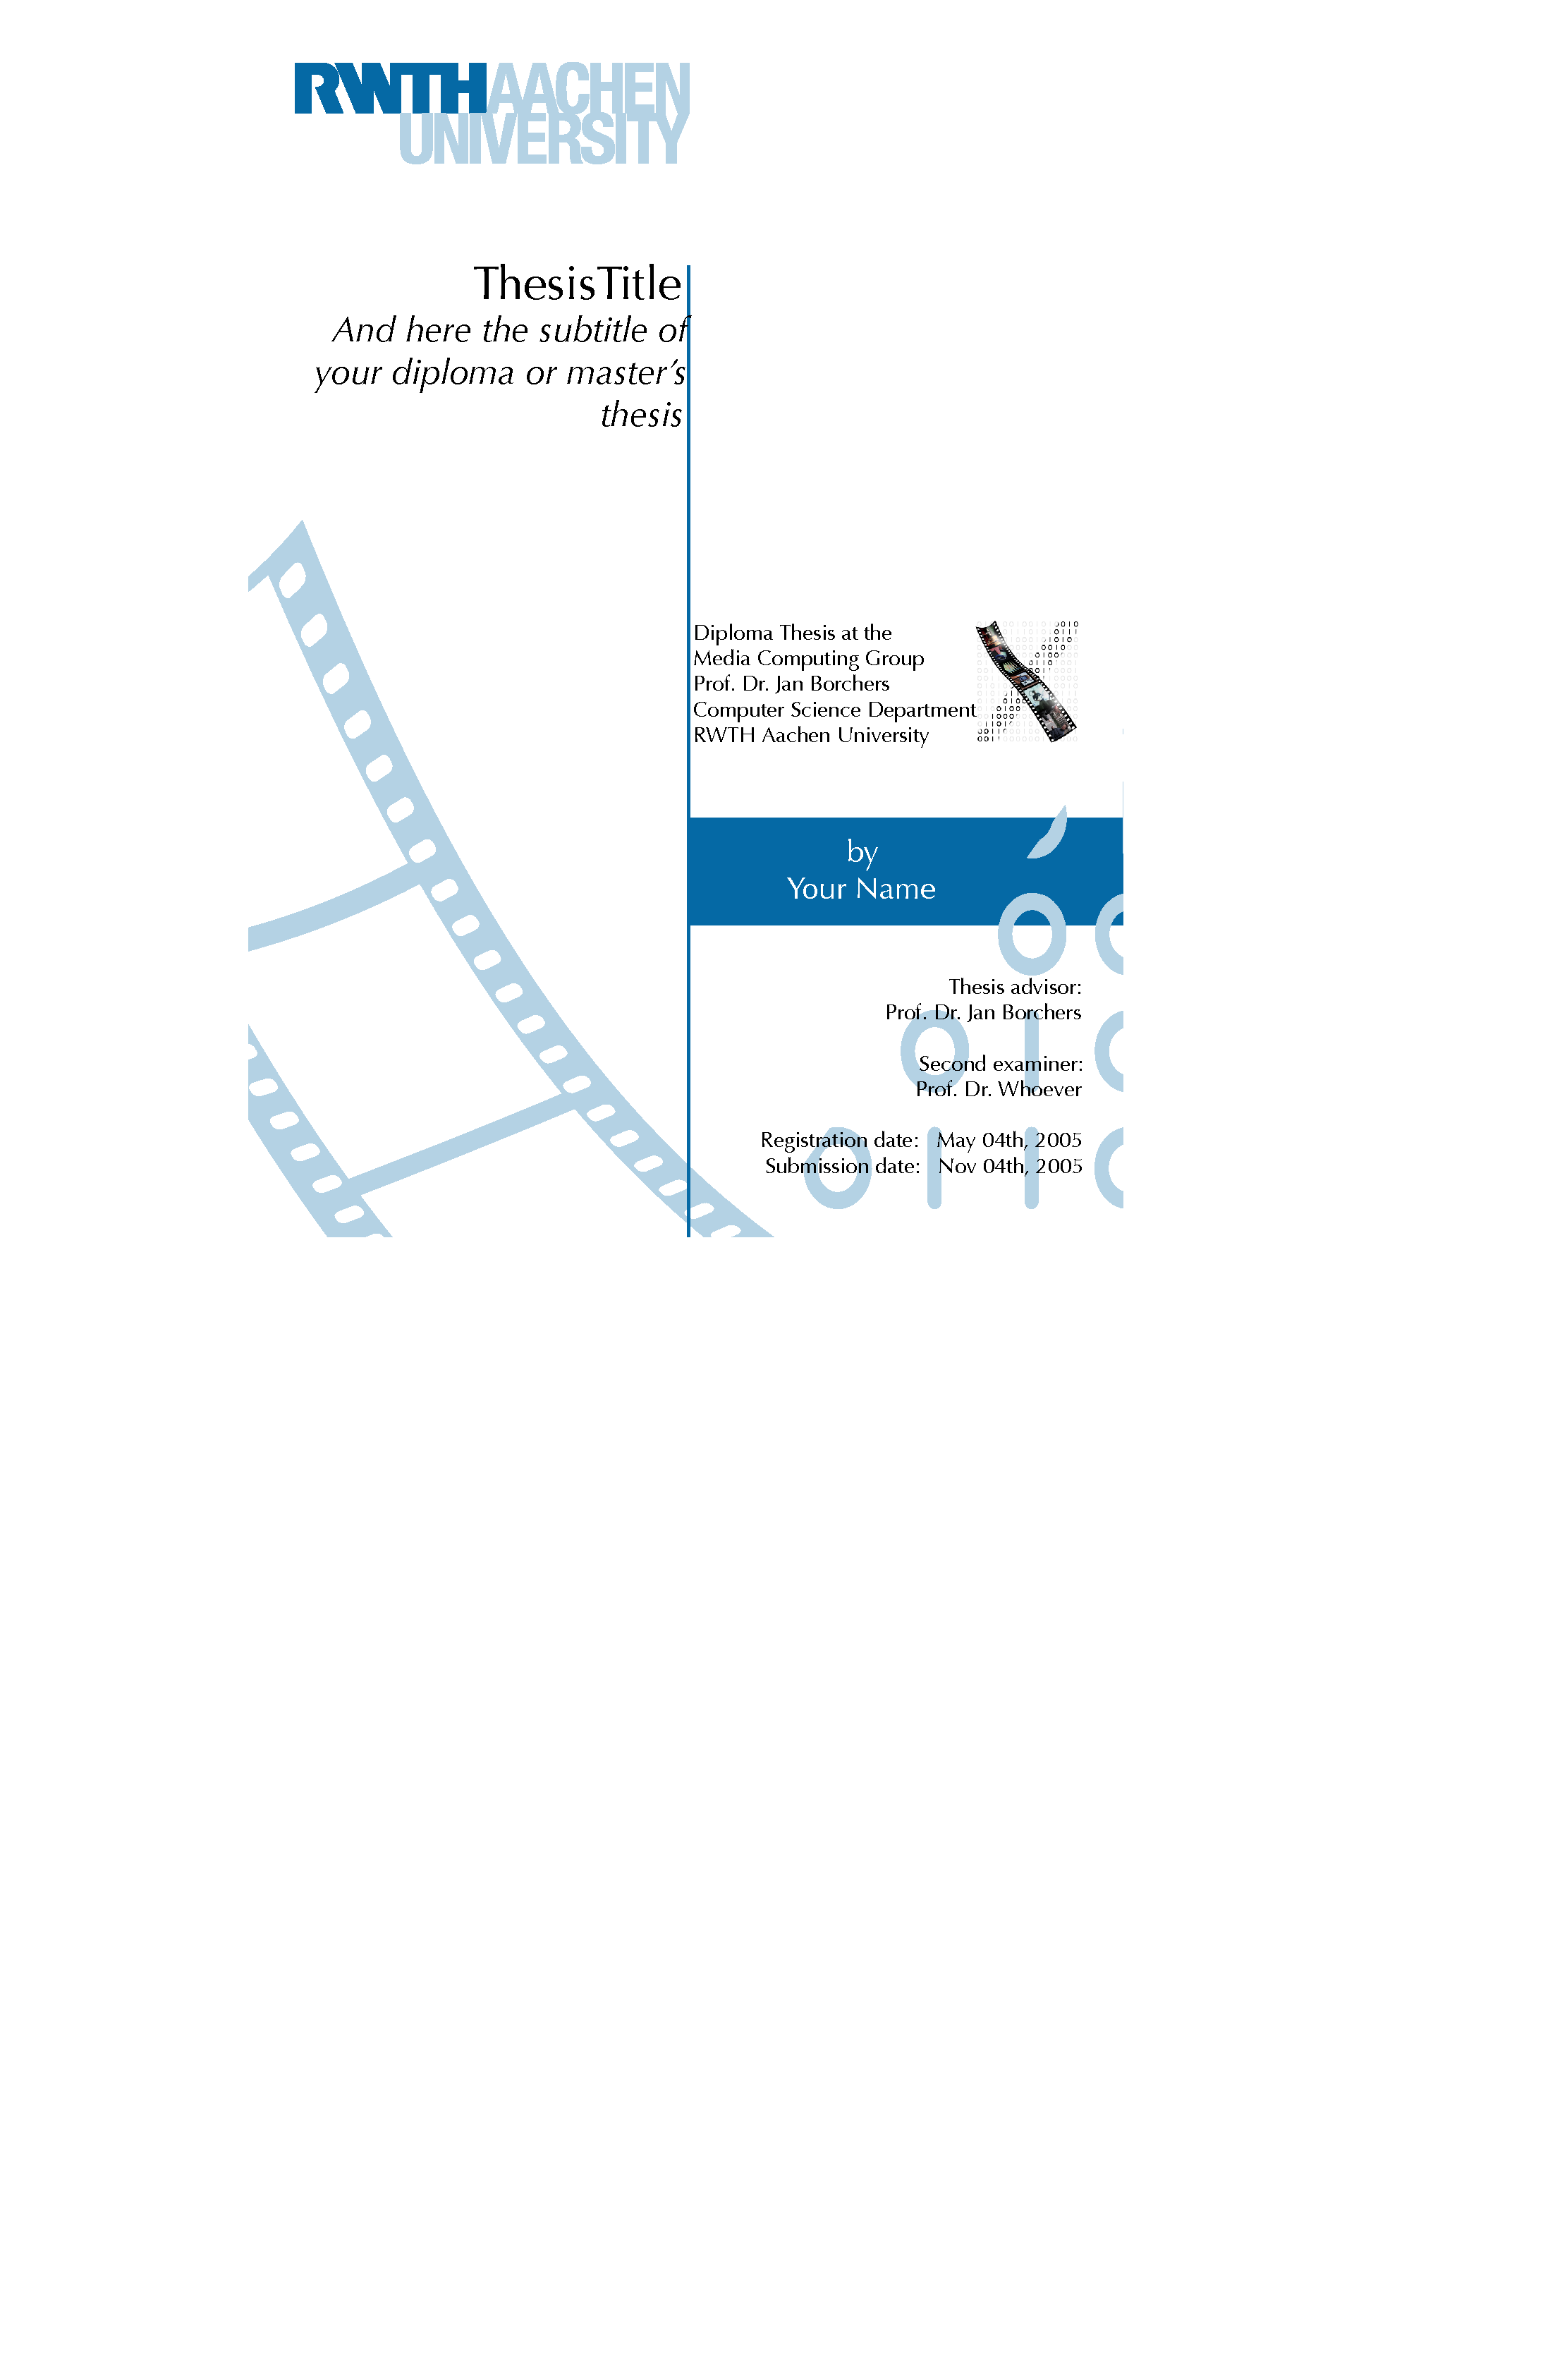
\includegraphics[width=\paperwidth]{titlepage}}}
\strut
\end{titlepage}

% This file is part of the i10 thesis template developed and used by the
% Media Computing Group at RWTH Aachen University.
% The current version of this template can be obtained at
% <http://www.media.informatik.rwth-aachen.de/karrer.html>.

~
\vfill
Layout based on a design by the Media Computing Group, RWTH Aachen University

 \url{http://hci.rwth-aachen.de/karrer_thesistemplate}


\emptydoublepage

% This file is part of the i10 thesis template developed and used by the
% Media Computing Group at RWTH Aachen University.
% The current version of this template can be obtained at
% <http://www.media.informatik.rwth-aachen.de/karrer.html>.

~
\vfill
I hereby declare that I have created this work completely on my own and used no other sources or tools than the ones listed, and that I have marked any citations accordingly.

Hiermit versichere ich, dass ich die vorliegende Arbeit selbst\"{a}ndig verfasst und keine anderen als die angegebenen Quellen und Hilfsmittel benutzt sowie Zitate kenntlich gemacht habe. 

\begin{flushright}
\vspace{12mm}
$\overline{Aachen, MONTH \mathit{YEAR}}$\\
\textit{YOUR NAME}
\end{flushright}

\emptydoublepage

\tableofcontents
\emptydoublepage
%
\listoffigures
\emptydoublepage
%
\listoftables
\emptydoublepage

%Die Übersicht sollte in englischer und in deutscher Sprache verfasst werden
%the abstract should include an english and a german version
% This file is part of the i10 thesis template developed and used by the
% Media Computing Group at RWTH Aachen University.
% The current version of this template can be obtained at
% <http://www.media.informatik.rwth-aachen.de/karrer.html>.

\chapter*{Abstract\markboth{Abstract}{Abstract}}
\addcontentsline{toc}{chapter}{\protect\numberline{}Abstract}
\label{abstract}

\begin{minipage}{\fullwidth}

%here (english version)

\end{minipage}



\chapter*{\"Uberblick\markboth{\"Uberblick}{\"Uberblick}}
\addcontentsline{toc}{chapter}{\protect\numberline{}\"Uberblick}
\label{ueberblick}

\begin{minipage}{\fullwidth}

%here (deutsche version)

\end{minipage}
\emptydoublepage

%Danksagungen
%acknowledgements
% This file is part of the i10 thesis template developed and used by the
% Media Computing Group at RWTH Aachen University.
% The current version of this template can be obtained at
% <http://www.media.informatik.rwth-aachen.de/karrer.html>.

\chapter*{Acknowledgements\markboth{Acknowledgements}{Acknowledgements}}
\addcontentsline{toc}{chapter}{\protect\numberline{}Acknowledgements}

\begin{minipage}{\fullwidth}

%Put your acknowledgements in here.
Thank you!

\end{minipage}


\emptydoublepage

%In der Arbeit verwendete Konventionen (Formelsatz, Definitionen, etc.)
%conventions applied in the thesis (AE/BE, definitions, etc.)
% This file is part of the i10 thesis template developed and used by the
% Media Computing Group at RWTH Aachen University.
% The current version of this template can be obtained at
% <http://www.media.informatik.rwth-aachen.de/karrer.html>.

\chapter*{Conventions\markboth{Conventions}{Conventions}}
\addcontentsline{toc}{chapter}{\protect\numberline{}Conventions}

Throughout this thesis we use the following conventions.



\bigskip

\emph{Text conventions}

Definitions of technical terms or short excursus are set off in coloured boxes.

\myDefBox{Excursus}
{Excursus are detailed discussions of a particular point in a book, usually in an appendix, or digressions in a written text.}

\medskip

Source code and implementation symbols are written in typewriter-style text.

\texttt{myClass}

\medskip

The whole thesis is written in Canadian English.

\medskip

Download links are set off in coloured boxes.

\myDownloadURL{File: myFile}{file_number.file}{file\myUnderscore number.file}

%\pagebreak

%\emph{Formula conventions}


\emptydoublepage

%--------------------------------------------------------------
\mainmatter

% This file is part of the i10 thesis template developed and used by the
% Media Computing Group at RWTH Aachen University.
% The current version of this template can be obtained at
% <http://www.media.informatik.rwth-aachen.de/karrer.html>.

\chapter{Introduction}
\label{introduction}

\begin{quotation}
After a long working day, Michael opens his apartment door. Or better, his door is opened for him. He has no key. Cameras at different positions in the corridor have registered his movement and his attitude. After entering his pin on a console, the DNA and the retina were scanned by another camera. An intelligent system has already approved him. As Michael enters the kitchen, his intelligent friend also sees that he is tired today. The light is dimmed, the blinds are shut down. Michael's behavior indicates that he does not want to be disturbed for the next hour. The phones and doorbell are switched to mute.

When Michael wakes up an hour later, he feels refreshed. The blinds open slightly. Michael now decides to do something for work as he often does, because he feels more relaxed there. He boots up his computer and opens the first working documents. The system is connected to the operating system of its job. It recognizes Michael's current and rapidly changing work processes. All other relevant and required information is provided discreetly while Michael starts listening to soft jazz and soul music. Michael begins to devote himself to his work.
\end{quotation}
The above scenario outlines a future working and private environment based on a networked intelligent system. It evokes reminiscences of \textit{HAL 9000}, the intelligent computer of Stanley Kubrick's Space Odysee 2001. \textit{HAL} is really intelligent, doing complex navigational computations for the spaceship and solving other computable problems. \textit{HAL} is sensitive, shows emotional reactions and bondings towards crew members, he is socialized and very human. Moreover, he is able to guess the intentions of the astronauts, knows their habits and has a strong drive for self-preservation. An emotional conflict forces him to draw his own conclusions, which lead to his deconstruction. As his neuronal circuits are slowly withdrawn from his artificial brain, \textit{HAL} suffers terribly. 

It is quite clear that intelligent machines will not be like this, but assistance and location based information systems are increasingly finding their way into everyday life. From a personal point of view, this development can be called either good or bad. Fact is, many representatives of \ac{AI} announce a quantum leap of  intelligent agents in the next decades, and more: Ray Kurzweil, Rodney Brooks, and Jeff Hawkins are of the opinion that the future of this development will be located in the so-called "'intelligent biological systems"', i.e. systems that replicate basic working principles of the brain. These will complement the previous learning-based inferential models for machine intelligence (\cite{kurzweil2013create},\cite{hawkins2007intelligence} and \cite{brooks2012brain}). 
But will these approaches be able to interpret emotions and guess about intentions? This is conceivable, if one thinks of the many sensors, which are described in the introductory example: A lower heart rate and blood pressure can indicate fatigue, facial expression can confirm this, etc. But without the physical sensors, this task gets difficult. Nevertheless, this is studied in computer science and slowly in psychology as well: How can we make sense of the "'actions"' of persons in the digital world, i.e. the websites searched, the documents read and the friends that were contacted? And moreover: Is this important at all?

Yes it is, and not just for the reason that social platforms and search engines like \textit{Facebook} and \textit{Google} gather and analyze a lot of personal data (it is always good to know, what others can do with private data). The main driving factor is the paradigm of the \textit{knowledge worker} that has become true for most of the western society and that proclaims a new working model:  The knowledge worker completes his tasks by non-routine problem-solving approaches with the help of a computer applications, the internet and social media (\cite{drucker1999knowledge}). As his work is fairly non-linear and complex, companies depend on these specialists (\cite{foss2006strategy}). In recent years the management boards of many companies became aware of this shift and established the position of a Chief Information Officers (CIO) whose work focus is information management. The objectives of this practical knowledge management go well beyond the mere supply of employes with relevant information: Employes are wanted to develop learning skills and abilities that provide added value for the company. The classification of knowledge is expressed on two poles: on the one hand the so-called explicit knowledge, which can be described and is therefore suitable to be kept in documents and on the other hand, implicit knowledge, which that can not be brought easily into tangible form. 

Getting implicit knowledge is studied in computer science under the term "'knowledge- and task mining"'. Its aim is to extract knowledge from elementary actions, i.e. operations on programs and documents, websites and social activities. 

This work tries to answer the question in what form knowledge can be extracted from interaction of users with the virtual environment. The concrete research questions are:

\fbox {
    \parbox{\linewidth}{
    \begin{enumerate}
      \item Is it possible to extract user tasks and intentions from state-of-art computer science approaches?
      \item What theoretical concepts of task analysis, goals and intentions are applied? What are the psychological foundations?
      \item If knowledge from elementary tasks can be extracted, how to handle that information?
    \end{enumerate}
    
    }
}

Questions 1. and 2. are answered in chapter \ref{relatedwork}. It will be argued that by the common approaches, so-called "'Intention-Aware Systems"' are not yet feasible. The theoretical shortcomings of the current concepts are revealed. As intentions are not extractable, there are two ways left to go. First, take existing approaches of computer science and see, how they can be integrated into organizations. Second try out a new approach and test, if the returned results are valuable and helpful on the way towards "'Intention-Aware Systems"'. The second way is handled by applying a new form of bio-inspired computing, called Hierarchical Temporal Memory (HTM), that will be explained in chapter XXX. Results will be compared to the findings of re-implemented traditional ways of knowledge-mining. 

The findings of either two approaches shall be evaluated and brought into organizational context to see, whether the extracted information is useful to a company. The evaluation and discussion are the last parts of this work.

 

\emptydoublepage
% This file is part of the i10 thesis template developed and used by the
% Media Computing Group at RWTH Aachen University.
% The current version of this template can be obtained at
% <http://www.media.informatik.rwth-aachen.de/karrer.html>.

\chapter{Related work}
\label{relatedwork}
\section{Knowledge and Task Mining}
In the computer scientific field of knowledge and task mining is no new subject.\mnote{Context-Aware Systems} With the rise of mobile computing devices the term context-aware systems was created. The meaning and definition are disputed. First publications referred to a user's location: in different places usually different contextual parameters are relevant. For example a diver that is ascending from deep water has to be made aware of resting times before emerging to the surface.Another example was the \textit{Active Badge Location System} in 1992 that detected the whereabouts of a person and in order to forward relevant phone calls to telephones close targeted person (\cite{want1992active}). Such systems adapt not only to the location but also to other relevant and changing parameters in the surroundings (\cite{schilit1994context}). This definition was widened in 1998 where context was referred to not only the computer accessible parameters of the surroundings but also the emotional state, focus of attention, date and time as well as people in the environment (\cite{dey1998context}). The new aspect of internal parameters like focus of attention was then referred to a further elaboration of the definition: the internal (logical) and external context: Internal context parameters are specified by the user in interaction with the computer like goals, tasks, work context, business processes and emotional state. External parameters are usually measured by hardware sensors, i.e. location, light, sound, movement, temperature, pressure etc. (\cite{hofer2003context}). The contextual parameters can be grouped into four categories: identity (marked by a unique identifier), the location (an entity’s position), activity (status, meaning the intrinsic properties of an entity, e.g., temperature and lightning for a room, processes running currently on a device etc.) and time (timestamps, \cite{dey2001conceptual}). An example of the use of internal data for extracting context is the \textit{Watson Project} \cite{budzik2000user}. Here the focus is shiftet for collecting contextual information from user interaction with the computer in order to proactively support the user. Proactivity is a term that  originates in organizational psychology and describes the ability of workers to not react to situations, but sense upcoming situational changes in advance and take control (\cite{grant2008dynamics}). As work gets more dependent of the retrieval and analysis of information, a proactive support system shall help the user in his various tasks by providing him with relevant information. This approach had further implications as gathering information from the user interaction with his computer requires techniques from information retrieval and computer linguistics. In this case the documents a user works with are analyzed and keywords are stored as vectors or a bag of words. The relevant keywords shall help to narrow the topical context a user is working on. Keywords than help to start searches with relevant search terms and provide the user with the information he needs (\cite{budzik2000user}). \mnote{Context-based Recommender Systems} As a single user is often not able to find the needed information, his typical search patterns are compared with those of other users. In these cases as \textit{user model} is created, and his search terms are compared to those of other users' and the documents they found. If keywords are matching, documents of those others users are recommended (\cite{anand2007contextual}). This approach is called context-based recommendation and their related techniques like user-collaborative filtering are applied in search engines like Amazon \footnote{www.amazon.com}. \textit{Attention-aware systems} at last have different focus: The guiding principle of Attention-aware systems is that users have limited cognitive resources and are distracted easily \mnote{Attention-aware systems}. They suffer from an \textit{information overload} as they jump quickly from one resource to the next in the same and different workings tasks. Whilst it is beneficial to be able to change foci in certain situations, in others it is exhausting. Therefore systems capable of supporting and guiding user attention have to assess the current user focus, and calculate the cost/benefits of attention shifts (interruptions). As this explanation shows, Attention-aware systems have a foundation in cognitive psychology. 

\emptydoublepage
% This file is part of the i10 thesis template developed and used by the
% Media Computing Group at RWTH Aachen University.
% The current version of this template can be obtained at
% <http://www.media.informatik.rwth-aachen.de/karrer.html>.

\chapter{Own work}
\label{ownwork} 
As was elaborated in the last chapter, an important research question is the detection of habits. This is based on the following findings:
\begin{itemize}
  \item Habits are stored as procedural knowledge structures in goal achievement. They are an indicator for expert knowledge as they free cognitive resources for more conscious intentional plans (\cite{aarts2000habits})
  \item Habits can predict future behavior (\cite{bentler1979models})
  \item Most activities of the day have habitual character  as they take place in the same context (social environment, people and preceding actions ((\cite{townsend2001sentence}, \cite{wood2007new})
  \item Habits usually are learned when achieving intentional goals but later, by a slow learning progress, they become subordinate parts of many goal directed behaviors (\cite{wood2007new}). 
\end{itemize}

It is interesting that the detection of habits has not yet been researched in computers sciences and even in psychology it is a relatively new subject as habits are hard to measure. The usual means for detecting patterns are diaries, self-reports or questionnaires. But habits are clearly behavioristic. Computers are an interesting platform to detect patterns. The following hypotheses are formulated:

\begin{itemize}
  \item Habits must be detectable by people who are involved with daily computer work
  \item Habits are an indicator for expert knowledge
  \item Habits can be predicted
  \item Habits indicate to relevant context parameters
\end{itemize}

The hypotheses rely on the ability to detect and measure habits. As chapter \ref{Model Human Processor} introduced, the \acf{MHP} and \acf{GOMS} are not feasible to detect tasks, but their methodical approaches can be used to analyze habits. This gets clearer as \ac{GOMS} was developed to estimate the total amount of time a task will take based on the composite of elementary actions. Routine cognitive skills can be described as a serial sequence of cognitive operations and motor activities. Each action can be quantified independently from the actual context. Figure \ref{fig6} shows the steps of a user by using his software: The user perceives activity on the screen, evaluates whether the activity is according to goals sets up the intention for the next step, retrieves the way to act accordingly on the system and executes his movements. The time for the activities is a compound empirical value of the \ac{MHP} where all operations are calculated from the interconnections of a set of processors and memories based on a "'recognize-act-cycle"': the "'perceptual processor"' encodes information from the senses to be available in the visual image  store (short-term memory). From there the encoded information is retrieved from the long-term memory that modifies the information in the short-term memory again (act of recognizing). After that, the decision to act is taken by the "'cognitive processor"' and executed by the "'motor processor"' (see chapter \ref{Model Human Processor}). As the feedback loop from action to perception is time-consuming, rapid acts are executed in bursts (\cite{card1986model}). The shortcomings of the \ac{GOMS} approach in elaborating tasks make it therefore useful for analyzing habits:

\begin{enumerate}
  \item The model applies only to very skilled users
  \item Learning or recall after periods of non-use are not elaborated
  \item The model focuses on errorless performance
  \item The model was developed exclusively for tasks in which the principal modeled components were assumed to be serial in nature
  \item The model does not address mental workload
  \item The model does not address fatigue
\end{enumerate}

Empirically derived values for typical actions were verified and are listed in table \ref{tab1}:
As time can vary for expert and novice mid-skilled users there is individual variation: For example key-stroke time for an average typist as is listed below is about $230$ msec. An expert writer is listed with $80$ msec (\cite{olson1990growth}).

\begin{table}[ht]
    \centering
    \begin{tabular}{lr} \toprule
    Type of action & Time \\ \midrule
    Enter a keystroke  & $230$ msec \\
    Point with a mouse  & $1500$ msec \\
    Move hands to mouse  & $360$ msec \\
    Perceive  & $100$ msec \\
    Retrieve from memory  & $1200$ msec \\
    Execute mental step  & $70$ msec \\
    Choose among methods  & $1250$ msec \\
    \bottomrule
\end{tabular}
 \caption{Cognitive engineering parameters}
 \label{tab1}
\end{table}

The sequences of burst actions can be described in the following manner: a skilled programmer is using an editor for writing code. He uses a many shortcuts (\textbf{sk}) and takes time to think (\textbf{M}) between busts of actions. A typical protocol of his text edits could look like the following
\begin{center}
  \textbf{<M,sk,sk,sk,M,sk,sk,sk>}
\end{center} 

Now the idea is, the programmer is very experienced. Shortcuts for him take about $150$ msec. Retrieval from memory takes about $1200$ msec. Total time for the burst action would be $ 2Ms + 6sks = 3200$ msec. The computer protocol on the other hand, would net detect the cognitive activities but the key presses. Therefore the protocol would exhibit 2 very quick bursts of action with a break of about one and a half seconds. 
Another example without using the keyboard: Imagine a knowledge worker clicking through menus in order to achieve his subtask like adding a table to a word document. He would have to move his mouse (\textbf{MM}) to the according main menu entry first: 'Insert' and click (\textbf{MC}), than he would choose the submenu entry: 'Table' and click (\textbf{MM,MC}). After that, a dialog pops up that lets the user choose the number of rows and columns. He moves his mouse to make to choose (\textbf{MM}) and then clicks to insert the table into his document (\textbf{MC}). The computer detected protocol could look like this:
\begin{center}
  \textbf{<MM,MC,MM,MC,MM,MC>}
\end{center} 

The total time would include the movement of the hand to the mouse at first and the cognitive operations. These are not included. But we can estimate the mouse click and mouse move time with roughly $1500$ msecs. The result would be $9000$ msec for the whole operation.

\emptydoublepage
% This file is part of the i10 thesis template developed and used by the
% Media Computing Group at RWTH Aachen University.
% The current version of this template can be obtained at
% <http://www.media.informatik.rwth-aachen.de/karrer.html>.

\chapter{Evaluation}
\label{evaluation}
\index{evaluation|(}

%here

 \index{evaluation|)}
\emptydoublepage
% This file is part of the i10 thesis template developed and used by the
% Media Computing Group at RWTH Aachen University.
% The current version of this template can be obtained at
% <http://www.media.informatik.rwth-aachen.de/karrer.html>.

\chapter{Summary and future work}
\label{summaryandfuturework}

%here

\section{Summary and contributions}
\label{summaryandfuturework.summary}

%here

\section{Future work}
\label{summaryandfuturework.futurework}
\index{future work|(}

%here

\index{future work|)}
\emptydoublepage

\begin{appendix}
% This file is part of the i10 thesis template developed and used by the
% Media Computing Group at RWTH Aachen University.
% The current version of this template can be obtained at
% <http://www.media.informatik.rwth-aachen.de/karrer.html>.

\chapter{TITLE OF THE FIRST APPENDIX}
\label{app.01}

\emptydoublepage
% This file is part of the i10 thesis template developed and used by the
% Media Computing Group at RWTH Aachen University.
% The current version of this template can be obtained at
% <http://www.media.informatik.rwth-aachen.de/karrer.html>.

\chapter{TITLE OF THE SECOND APPENDIX}
\label{app.02}


\emptydoublepage
\end{appendix}

%--------------------------------------------------------------
\backmatter

%acronyms
\clearpage
\include{acronyme}

%Bibliographie
%bibliography
\clearpage
\addcontentsline{toc}{chapter}{\protect\numberline{}Bibliography}
\bibliography{../literature/knowledge}
\emptydoublepage

%Index
%index
\markboth{Index}{Index}
\thispagestyle{plain}
\addcontentsline{toc}{chapter}{\protect\numberline{}Index}
\printindex

%Satzdatum
%date of typesetting
\newpage
\thispagestyle{empty}
\vspace*{\fill}
\hspace*{\fill}{\tiny Typeset \today}

%--------------------------------------------------------------
\end{document}
